\documentclass[letterpaper,  %a4paper
               %boxit,
               %titlepage,   % separate title page
               %refpage      % separate references
              ]{jacow-2_3}   %jacow}
%
% CHANGE SEQUENCE OF GRAPHICS EXTENSION TO BE EMBEDDED
% ----------------------------------------------------
% test for XeTeX where the sequence is by default eps-> pdf, jpg, png, pdf, ...
%    and the JACoW template provides JACpic2v3.eps and JACpic2v3.jpg which
%    might generates errors, therefore PNG and JPG first
%
\makeatletter%
	\ifboolexpr{bool{xetex}}
	 {\renewcommand{\Gin@extensions}{.pdf,%
	                    .png,.jpg,.bmp,.pict,.tif,.psd,.mac,.sga,.tga,.gif,%
	                    .eps,.ps,%
	                    }}{}
\makeatother

% CHECK FOR XeTeX/LuaTeX BEFORE DEFINING AN INPUT ENCODING
% --------------------------------------------------------
%   utf8  is default for XeTeX/LuaTeX 
%   utf8  in LaTeX only realizes a small portion of codes
%
\ifboolexpr{bool{xetex} or bool{luatex}} % test for XeTeX/LuaTeX
 {}                                      % input encoding is utf8 by default
 {\usepackage[utf8]{inputenc}}           % switch to utf8

\usepackage[USenglish]{babel}			 

\usepackage[final]{pdfpages}
\usepackage{multirow}
\usepackage{ragged2e}
\usepackage{tikz}
\usetikzlibrary{shapes,arrows,backgrounds}
\usetikzlibrary{mindmap,trees}
\usetikzlibrary{decorations.pathreplacing}
\usetikzlibrary{plotmarks}
%
% if BibLaTeX is used
%
\ifboolexpr{bool{jacowbiblatex}}%
 {%
  \addbibresource{jacow-test.bib}
  \addbibresource{biblatex-examples.bib}
 }{}
\listfiles

%
% command for typesetting a \section like word
%
\newcommand\SEC[1]{\textbf{\uppercase{#1}}}

%%
%%   Lengths for the spaces in the title
%%   \setlength\titleblockstartskip{..}  %before title, default 3pt
%%   \setlength\titleblockmiddleskip{..} %between title + author, default 1em
%%   \setlength\titleblockendskip{..}    %afterauthor, default 1em

%\copyrightspace %default 1cm. arbitrary size with e.g. \copyrightspace[2cm]

% testing to fill the copyright space
%\usepackage{eso-pic}
%\AddToShipoutPictureFG*{\AtTextLowerLeft{\textcolor{red}{COPYRIGHTSPACE}}}

\begin{document}

\title{Bunch length measurements using CTR at the AWA with comparison to simulation}

\author{N. Neveu\textsuperscript{1}\thanks{nneveu@anl.gov}, 
	    L. Spentzouris, Illinois Institute of Technology, Chicago, IL, USA \\
		A. Halavanau, P. Piot\textsuperscript{2}, Northern Illinois University, DeKalb, IL, USA \\
		\textsuperscript{2} also at Fermilab, Batavia, IL, USA \\
		S. Antipov, Euclid Techlabs LLC, Solon, OH, USA \\
	    J. G. Power, E. Wisniewski, C. Whiteford, \textsuperscript{1}Argonne National  Laboratory, Lemont, IL, USA \\
	    }
\maketitle

%
\begin{abstract}
In this paper we present electron bunch length measurements 
at the Argonne Wakefield Accelerator (AWA) photoinjector facility. 
The AWA accelerator has a large dynamic charge density range, 
with electron beam charge varying between 0.1 nC - 100 nC, 
and laser spot size diameter at the cathode between 0.1 mm - 18 mm. 
The bunch length measurements were taken at different charge densities 
using a metallic screen and a Martin-Puplett interferometer to perform 
autocorrelation scans of the corresponding coherent transition radiation (CTR). 
A liquid helium-cooled 4K bolometer was used to register the interferometer signal. 
The experimental results are compared with OPAL-T numerical simulations.
\end{abstract}


\section{AWA Facility}
The AWA Facility houses two rf photoinjectors, both 
operating at \SI{1.3}{GHz}. The photoinjector used for 
these studies consists of a gun and solenoids followed
by six accelerating cavities, as shown in Fig.~\ref{beamline}. 
This beam line is capable of low (\SI{0.1}{nC}) and 
high charge (\SI{100}{nC}) operation.
Both beamlines utilize the 248 nm UV laser 
to generate photoelectrons with the Full Width Half Maximum
(FWHM) pulse duration ranging from 1.5 ps to 10 ps.
The bunch charge is 
routinely adjusted depending on the requirements 
of the experiments downstream of the photoinjector.
Typical operating charges are 1, 4, 10, and \SI{40}{nC}. 
While these are the most
common operating modes, other charges have been requested 
and provided depending on the experiment.
Recent experiments include emittance exchange \cite{eex}, 
structure tests \cite{pets}, thermal emittance measurements \cite{therm}, 
and two beam acceleration \cite{tba}. 
Recently, AWA laser system was upgraded with a microlens array (MLA) setup
that yields very transversely homogeneous bunches \cite{PhysRevAccelBeams.20.103404}.
The effect of the MLA generated beam on the final electron 
bunch length had not been investigated, motivating this work.



\section{Measurement Technique}
In order to measure the bunch length, we performed an autocorrelation scan
of the CTR produced by the electron distribution \cite{Happek, WBarry}.
In brief, the CTR is transported into a Martin-Puplett interferometer (MPI)
where it's split and directed into two MPI arms with a half-transparent pellicle \cite{PhysRevSTAB.9.082801}. 
The CTR beams are then combined together at the exit of the MPI with the variable path difference.
The resulting CTR intensity is registered with a liquid helium cooled IR Labs
bolometer \cite{IRlabs} as a function of path difference.
The path difference is then converted into time as $\Delta \tau = 2 \Delta x$.
The resulting FWHM bunch duration is determined from the Gaussian fit of 
the interferogram; see Fig. \ref{interferogram}.
\begin{figure}
 \includegraphics[width=1.0\linewidth]{images/measurement}
 \caption{An example interferogram for Q=30 nC and laser pulse FWHM of 1.5 ps.}
 \label{interferogram}
\end{figure}
To alleviate the effect of charge fluctuations, we recorded 15 bolometer values for each data point.
The values were then averaged and the errorbars were deduced from the data. The data points
outside of the 3$\sigma$ bracket were considered as outliers and discarded. The resulting
interference pattern as a function of time delay in the MPI is similar to that presented in Fig.~\ref{interferogram}.

\begin{figure*}[hbt]
	\centering
	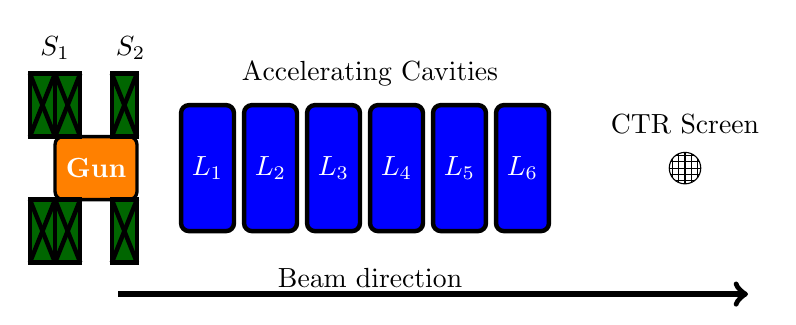
\begin{tikzpicture}[scale=0.8, text=black]
	\def \gunleft {-1.0}
\def \gunright {0.3}
\def \loneright {1.0}
\def \ltworight {2.0}
\def \lthreeright {3.0}
\def \lfourright {4.0}
\def \lfiveright {5.0}
\def \lsixright {6.0}
\def \quadone {7.5}

%Line between kicker and septum
\node[] at (4.0,-0.75) {Beam direction};
\draw[line width=0.75mm, ->] (0.0,-1.0) -- (10,-1.0);

\draw[fill=orange, very thick, rounded corners =0.1cm] (\gunleft,0.5)rectangle (\gunright,1.5) node[pos=.5, white] {\textbf{Gun}} ;
%S1
\node[] at (-1,2.9) {$S_1$};
\draw[ultra thick, fill=black!60!green] (-1.4,-0.5)rectangle  (-1.0,0.5) node[pos=.5, white] {} ;
\draw[black, ultra thick] (-1.4,-0.5) -- (-1.0,0.5);
\draw[black, ultra thick] (-1.4,0.5) -- (-1.0,-0.5);
\draw[ultra thick, fill=black!60!green] (-1.4,1.5)rectangle  (-1.0,2.5) node[pos=.5, white] {} ;
\draw[black, ultra thick] (-1.4,1.5) -- (-1.0,2.5);
\draw[black, ultra thick] (-1.4,2.5) -- (-1.0,1.5);
%S2
\draw[ultra thick, fill=black!60!green] (-1.0,-0.5)rectangle  (-0.6,0.5) node[pos=.5, white] {} ;
\draw[black, ultra thick] (-1.0,-0.5) -- (-0.6,0.5);
\draw[black, ultra thick] (-1.0,0.5) -- (-0.6,-0.5);
\draw[ultra thick, fill=black!60!green] (-1.0,1.5)rectangle  (-0.6,2.5) node[pos=.5, white] {} ;
\draw[black, ultra thick] (-1.0,1.5) -- (-0.6,2.5);
\draw[black, ultra thick] (-1.0,2.5) -- (-0.6,1.5);

%S3
\node[] at (0.2,2.9) {$S_2$};
\draw[ultra thick, fill=black!60!green] (-0.1,-0.5) rectangle  (0.3,0.5) node[pos=.5, white] {};
\draw[black, ultra thick] (-0.1,-0.5) -- (0.3,0.5);
\draw[black, ultra thick] (-0.1,0.5) -- (0.3,-0.5);
\draw[ultra thick, fill=black!60!green] (-0.1,1.5) rectangle  (0.3,2.5) node[pos=.5, white] {};
\draw[black, ultra thick] (-0.1,1.5) -- (0.3,2.5);
\draw[black, ultra thick] (-0.1,2.5) -- (0.3,1.5);
%Linac drawings 
\node[] at (4,2.5) {Accelerating Cavities};
\draw[fill=blue, ultra thick, rounded corners =0.1cm] (\loneright,0)rectangle  ({\loneright+0.84},2) node[pos=.5, white] {$L_1$} ;
\draw[fill=blue, ultra thick, rounded corners =0.1cm] (\ltworight,0)rectangle  ({\ltworight+0.84},2) node[pos=.5, white] {$L_2$};
\draw[fill=blue, ultra thick, rounded corners =0.1cm] (\lthreeright,0)rectangle ({\lthreeright+0.84},2) node[pos=.5, white] {$L_3$};
\draw[fill=blue, ultra thick, rounded corners =0.1cm] (\lfourright,0)rectangle ({\lfourright+0.84},2) node[pos=.5, white] {$L_4$};
\draw[fill=blue, ultra thick, rounded corners =0.1cm] (\lfiveright,0)rectangle ({\lfiveright+0.84},2) node[pos=.5, white] {$L_5$};
\draw[fill=blue, ultra thick, rounded corners =0.1cm] (\lsixright,0)rectangle ({\lsixright+0.84},2) node[pos=.5, white] {$L_6$};



%current optimization point
%\node[draw, fill=yellow, star, star points=5, star point ratio=0.6, minimum size=0.1cm]
%at (12.5,1.0) {$z_1$};
\node[] at (9,1.7) {CTR Screen};
\clip[draw] (9,1) circle (0.25cm);
\draw[step=1mm] (-1,-1) grid (10,10);



%\draw[latex-latex] (\gunleft,-5.0) -- (14,-5.0) ;
%\foreach \x in  {0.3, 1.0, 3.5, 5.0, 7.0, 8.5, 10, 12.5} %tick marks
%\draw[shift={(\x,-5.0)},color=black] (0pt,3pt) -- (0pt,-3pt);
%\foreach \x in {0.3, 1.0, 3.5, 5.0, 7.0, 8.5, 10, 12.5}
%\draw[shift={(\x,-5.2)},color=black] (0pt,0pt) node[below] {$\x$};

%Line between kicker and septum
\draw[very thick] (13.25,0.2) -- (14.5,-0.5);


%Line between septum and dipole
\draw[very thick] (15.6,-0.5) -- (16.5,-0.5);




	\end{tikzpicture}	
	\caption{Beam line layout at the AWA.}
	\label{beamline}
\end{figure*}
\section{Experimental Setup}
The beam line layout is shown in Fig.~\ref{beamline}. 
Bunches were allowed to propagate freely to the 
CTR screen. The only focusing elements used were solenoids $S_1$ and
$S_2$. As the bunches passed the CTR screen, light was
emitted through a window located next to the screen, 
as shown in Fig.~\ref{bolo}. A slit was used to prevent
background x-rays from reaching the bolometer.
After passing the slit, the CTR propagated to the 
 interferometer also shown in Fig.~\ref{bolo}. 
A remotely movable stage inside the interferometer was swept, 
and the resulting combined signal fed to the bolometer. 
%The bolometer was cooled with liquid helium. 
Periodic refilling of the helium was required throughout the day in order
to keep the bolometer at \SI{4}{K}. The bolometer sensitivity knob was at position ``1'' and
the gain set to 200.
For the case of 1 nC electrons beams, the laser transverse profile was homogenized prior to the vacuum injection \cite{PhysRevAccelBeams.20.103404}.
To produce high-charge 40 nC beams, we implemented an additional laser beamline that bypasses the homogenizer due to the losses in the 
MLA and relay optics.



\begin{figure}
	\begin{tikzpicture}[every node/.style={anchor=south west,inner sep=0pt},x=1mm, y=1mm,]   
	\node (fig1) at (0,0)
	{\includegraphics[width=0.5\textwidth]{images/interferometer}};
	\node[fill=white, inner sep=2pt] (txt2) at (35,15) {Interferometer};
	\node[fill=white, inner sep=2pt, rotate=26] (txt2) at (18,19.5) {Slit};	
	\node[fill=white, inner sep=2pt, rotate=20] (txt2) at (13,27) {Window};

	\node (fig2) at (0,-50)
	{\includegraphics[width=0.5\textwidth]{images/bolometer}};
	\node[fill=white, inner sep=2pt] (txt2) at (35,-42) {Interferometer};	
	\node[fill=white, inner sep=2pt] (txt2) at (55,-25) {Window};	
	\node[fill=white, inner sep=2pt] (txt2) at (22,-15) {Bolometer};
	\end{tikzpicture}
	\caption{IR labs bolometer and MPI interferometer used in the experiment
		 to capture CTR light as it exited a window on the beam line. }
	%\label{inter}
	%\caption{Bolometer. }
	\label{bolo}
\end{figure}


\section{Simulations}
Simulations of the AWA beam line shown in Fig.~\ref{beamline}
were performed with the code and OPAL~\cite{opal}.
The gun, accelerating cavities, and solenoids were modeled with 2D
Poisson/Superfish~\cite{fish} files. All field maps were in the T7 format.
Input parameters for the simulations are shown in Table~\ref{simparam}.
Note that on crest refers to the phase of max energy gain.
In the case of the gun, a -~$5^{\circ}$ phase is measured 
w.r.t the peak rf voltage.
\begin{table}[hbt]
	%   \vspace*{-.5\baselineskip}
	\centering
	\caption{Simulation Parameters}
	\begin{tabular}{lcc}
		\toprule
		\textbf{Parameter} & \textbf{Low Charge}  & \textbf{High Charge} \\
		\midrule
		Charge       & 0.3, 0.7, \SI{1.3}{nC}        & \SI{40}{nC}    \\ %[3pt]
		Gun Gradient & \SI{65}{MV/m}     & \SI{65}{MV/m}  \\ %[3pt]
		Gun Phase    & \SI{0}{}$^{\circ}$ & \SI{-5}{}$^{\circ}$ \\		 
		$S_1$        & \SI{230}{A}		 & \SI{500}{A}	  \\
		$S_2$		 & \SI{150}{A}   	 & \SI{235}{A}		 \\
		Linac Phases & On crest          & On crest       \\
		Laser FWHM   & \SI{1.5}{ps}      & \SI{1.5}{ps}   \\ %[3pt]
		Laser Radius & \SI{2}{mm}        & \SI{9}{mm}     \\
		\bottomrule
	\end{tabular}
	\label{simparam}
	%   \vspace*{-\baselineskip}
\end{table}

Four scenarios were simulated, three low charge cases at 0.3, 0.7, and \SI{1}{nC}, and a 
high charge case at \SI{30}{nC}. 
These charges and input parameters were specifically chosen to 
match experimental measurements that had taken place or would 
take place in the future. Each simulation was run with 10,000 particles 
on 8 cores, and ran 2.5 minutes to reach a z location of \SI{17}{m}.
Prior work \cite{benchmark} indicates the bunch length is not 
very sensitive to the number of particles or grid size. 
This would not be the case if we were comparing emittance, or 
transverse characteristics. We expected charge, energy,
and laser parameters to have the most impact on the simulation values.


\section{Results}
Comparison of simulation and experimental results are shown in Fig.~\ref{sims}.
\begin{figure*}[!tbh]
	\centering
	\includegraphics[width=0.8\linewidth]{images/bunchlength}
	\caption{Comparison of simulations and experimental measurements.}
	\label{sims}
\end{figure*}
While, we do not have an exact match, the results agree within reason.
The discrepancies indicate there are still adjustments that can be made
to the simulation model. We will continue to try to improve agreement
as more of these measurements are made. 
This can include better measurements of the beam energy, and careful attention to other 
beam line parameters such as the laser radius and solenoid strengths.
In the case of high charge simulations, where the agreement is the worst, 
more consideration is needed for large charge fluctuations in the data.

Experimentally measured values of the bunch duration are shown in Table~\ref{exp}.
Note the units in the table are picoseconds and the units in Fig.~\ref{sims} are millimeters.
The table gives bunch duration, and the plot gives bunch length for the same data.
We hope these can serve as future reference for others doing experiments at the AWA.
\begin{table}[h]
	\centering
	\caption{Experimental Measurements}
	\begin{tabular}{rcc}
		\toprule
		\textbf{Charge} & \textbf{Bunch Dur. (RMS)} & \textbf{Laser spot size}  \\
		\midrule
		\SI{0.3}{nC} & \SI{2.2}{ps} & 4 mm    \\ %[3pt]
		\SI{0.7}{nC} & \SI{2.6}{ps} & 4 mm   \\ %[3pt]
		\SI{1.3}{nC} & \SI{2.6}{ps} & 4 mm    \\
		\SI{30}{nC}  & \SI{4.1}{ps} & 9 mm \\ %[3pt]
		\bottomrule
	\end{tabular}
	\label{exp}
\end{table}


\section{Conclusion}
We performed experimental measurements of the electron bunch 
length using CTR and scanning interferometer technique.
The data was analyzed and compared to OPAL simulations.
The bunch length for the cases of 1 and \SI{30}{nC} is reported.
We note a decent agreement between the simulations and 
experimental results. The experimental setup will be used in the future
AWA CTR studies. 



\section{acknowledgments}
We would like to thank 
Northern Illinois University (NIU) for providing the 
interferometer used in this experiment. The work of A.H. 
is supported by the US Department of Energy under contract No. DE-SC0011831 with Northern Illinois University.
We also gratefully acknowledge the computing resources
provided on Bebop, a high-performance computing cluster
operated by the LCRC at Argonne National Laboratory.
This material is based upon work supported by the 
U.S. Department of Energy, Office of Science, under 
contract number DE-AC02-06CH11357 and grant number DE-SC0015479. 
Travel to IPAC'18 supported by the United States National Science Foundation, 
the Division of Physics of Beams of the American Physical Society, and TRIUMF.


\begin{thebibliography}{99}
\bibitem{eex}
G.~Ha \emph{et al.}, “Demonstration of Current Profile 
Shaping using Double Dog-Leg Emittance Exchange Beam 
Line at Argonne Wakefield Accelerator”
in \textit{Proc. IPAC’16}, 
Busan, South Korea, May 2016, 
paper TUOBB01.

\bibitem{pets}
J.~Shao \emph{et al.}, 
“Recent Progress towards Dielectric Short Pulse Two-Beam Acceleration”
in \textit{Proc. IPAC’18}, 
Vancouver, Canada, May 2018, 
paper TUYGBE3.

\bibitem{therm}
L.~Zheng \emph{et al.}, “Measurements of Thermal Emittance 
for Cesium Telluride Photocathodes in an L-Band RF Gun”
in \textit{Proc. IPAC’17}, 
Copenhagen, Denmark, May 2017, 
paper TUPAB074.

\bibitem{tba}
J.~Shao \emph{et al.}, “Recent Two-Beam 
Acceleration Activities at Argonne Wakefield Accelerator Facility”
in \textit{Proc. IPAC’17}, 
Copenhagen, Denmark, May 2017, 
paper WEPVA022.

\bibitem{PhysRevAccelBeams.20.103404}
A.~Halavanau \textit{et al.},
%"Spatial Control of Photoemitted Electron Beams using a Micro-Lens-Array Transverse-Shaping Technique",
\emph{Phys. Rev. Accel. Beams}, 20:103404, 2017.

\bibitem{Happek}
U.~Happek, A.~J. Sievers, and E.~B. Blum,
%\newblock "Observation of coherent transition radiation",
\emph{Phys. Rev. Lett.}, 67:2962--2965, (1991).

\bibitem{WBarry}
W. Barry,
%\newblock "Measurement of subpicosecond bunch profiles using coherent transition radiation",
\emph{AIP Conference Proceedings}, 390(1):173--185, 1997.

\bibitem{PhysRevSTAB.9.082801}
D.~Mihalcea, C.~L. Bohn, U.~Happek, and P.~Piot,
%\newblock "Longitudinal electron bunch diagnostics using coherent transition radiation",
\newblock \emph{Phys. Rev. ST Accel. Beams}, 9:082801, (2006).

\bibitem{IRlabs}
IR~Labs,
\newblock \url{http://www.infraredlaboratories.com/home.html}

\bibitem{opal}
A.~Adelmann \emph{et al.},
“The OPAL (Object Oriented Parallel Accelerator Library) framework,”
PSI, Zurich, Switzerland,
Rep. PSI-PR-08-02, 2008-2017.

\bibitem{fish}
\emph{Reference Manual for the POISSON/SUPERFISH Group of 
	Codes},  Los Alamos Accelerator Code Group,  
Los Alamos, NM, USA, 
Rep. LA-UR-87-126, Jan. 1987.

\bibitem{benchmark}
N.~Neveu \emph{et al.}, 
“Benchmark of RF Photoinjector and Dipole
Using ASTRA, GPT, and OPAL”
in \textit{Proc. NAPAC’16}, 
Chicago, IL, USA, Oct. 2016, 
paper THPOA46.




\end{thebibliography}



\null  % this is a hack for correcting the wrong un-indent by package 'flushend' in versions before 2015




\end{document}
